% A0 landscape poster (tikzposter). Upload this folder to Overleaf as its own project and compile with pdfLaTeX.
% For portrait, remove "landscape" and change the column widths below.
\documentclass[25pt, a0paper, landscape, margin=15mm, innermargin=15mm, blockverticalspace=12mm, colspace=12mm, subcolspace=8mm]{tikzposter}

\usepackage{graphicx}
\usepackage{booktabs}
\usepackage{qrcode}
\usepackage[T1]{fontenc}
\usepackage{helvet}
\renewcommand{\familydefault}{\sfdefault}

\usetheme{Default}
\usecolorstyle[colorPalette=BlueGrayOrange]{Germany}
\colorlet{titlebgcolor}{white}   % light title box; text set to the palette blue below
\makeatletter
\settitle{%
  \begin{minipage}[c]{0.78\textwidth}\centering
    {\color{colorOne}\fontsize{68}{82}\selectfont\bfseries What Limits Mechanical-Axis Accuracy in Full-Length\\
      Femur Reconstruction from Biplanar Radiographs?\par}\vspace{0.6em}
    {\huge \@author\par}\vspace{0.3em}
    {\LARGE \@institute\par}
  \end{minipage}\hfill
  \begin{minipage}[c]{0.12\textwidth}\centering
    \qrcode[height=9cm]{https://github.com/ayyp1/biplanar-xray-to-3d-femur}\\[0.3em]
    {\large code \& weights}
  \end{minipage}}
\makeatother

\title{What Limits Mechanical-Axis Accuracy in Full-Length Femur Reconstruction from Biplanar Radiographs?}
\author{Ashish Kumar Pokharel}
\institute{ashishkumar.pokharel@gmail.com \quad$\cdot$\quad github.com/ayyp1/biplanar-xray-to-3d-femur}

\newcommand{\claim}[1]{{\large\bfseries #1}\par\vspace{0.4em}}
\tikzposterlatexaffectionproofoff
\begin{document}
\maketitle[width=0.96\textwidth]

\begin{columns}

% ---------------------------------------------------------------- column 1
\column{0.30}
\block{Question}{
  The \textbf{femoral mechanical axis} (hip centre $\rightarrow$ knee centre) guides osteotomy and arthroplasty
  planning. Deep networks can rebuild the femur in 3D from two radiographs, but are usually judged by \textbf{Dice}
  on the proximal femur.

  \vspace{0.5em}
  \claim{What actually limits the accuracy of the axis: the network, the reconstruction, or the landmarks?}
}

\block{Data and Method}{
  \begin{itemize}
    \item \textbf{HFValid}: 101 whole-femur CTs with expert surfaces and landmarks, 5-fold cross-validation.
    \item \textbf{VSD} (external): 58 femurs; 19 with 5 raters $\times$ 4 repetitions.
    \item Synthetic AP + lateral radiographs (DRRs, 2\,mm), fused into one 3D input.
    \item \textbf{AttentionUNet} (1.5M) vs \textbf{SwinUNETR} (62M), identical folds, four training configurations.
    \item Hip: sphere fit; knee: widest level + offset. \textbf{Floor} = same extractor on the true masks.
  \end{itemize}
  \vspace{0.5em}
  \centering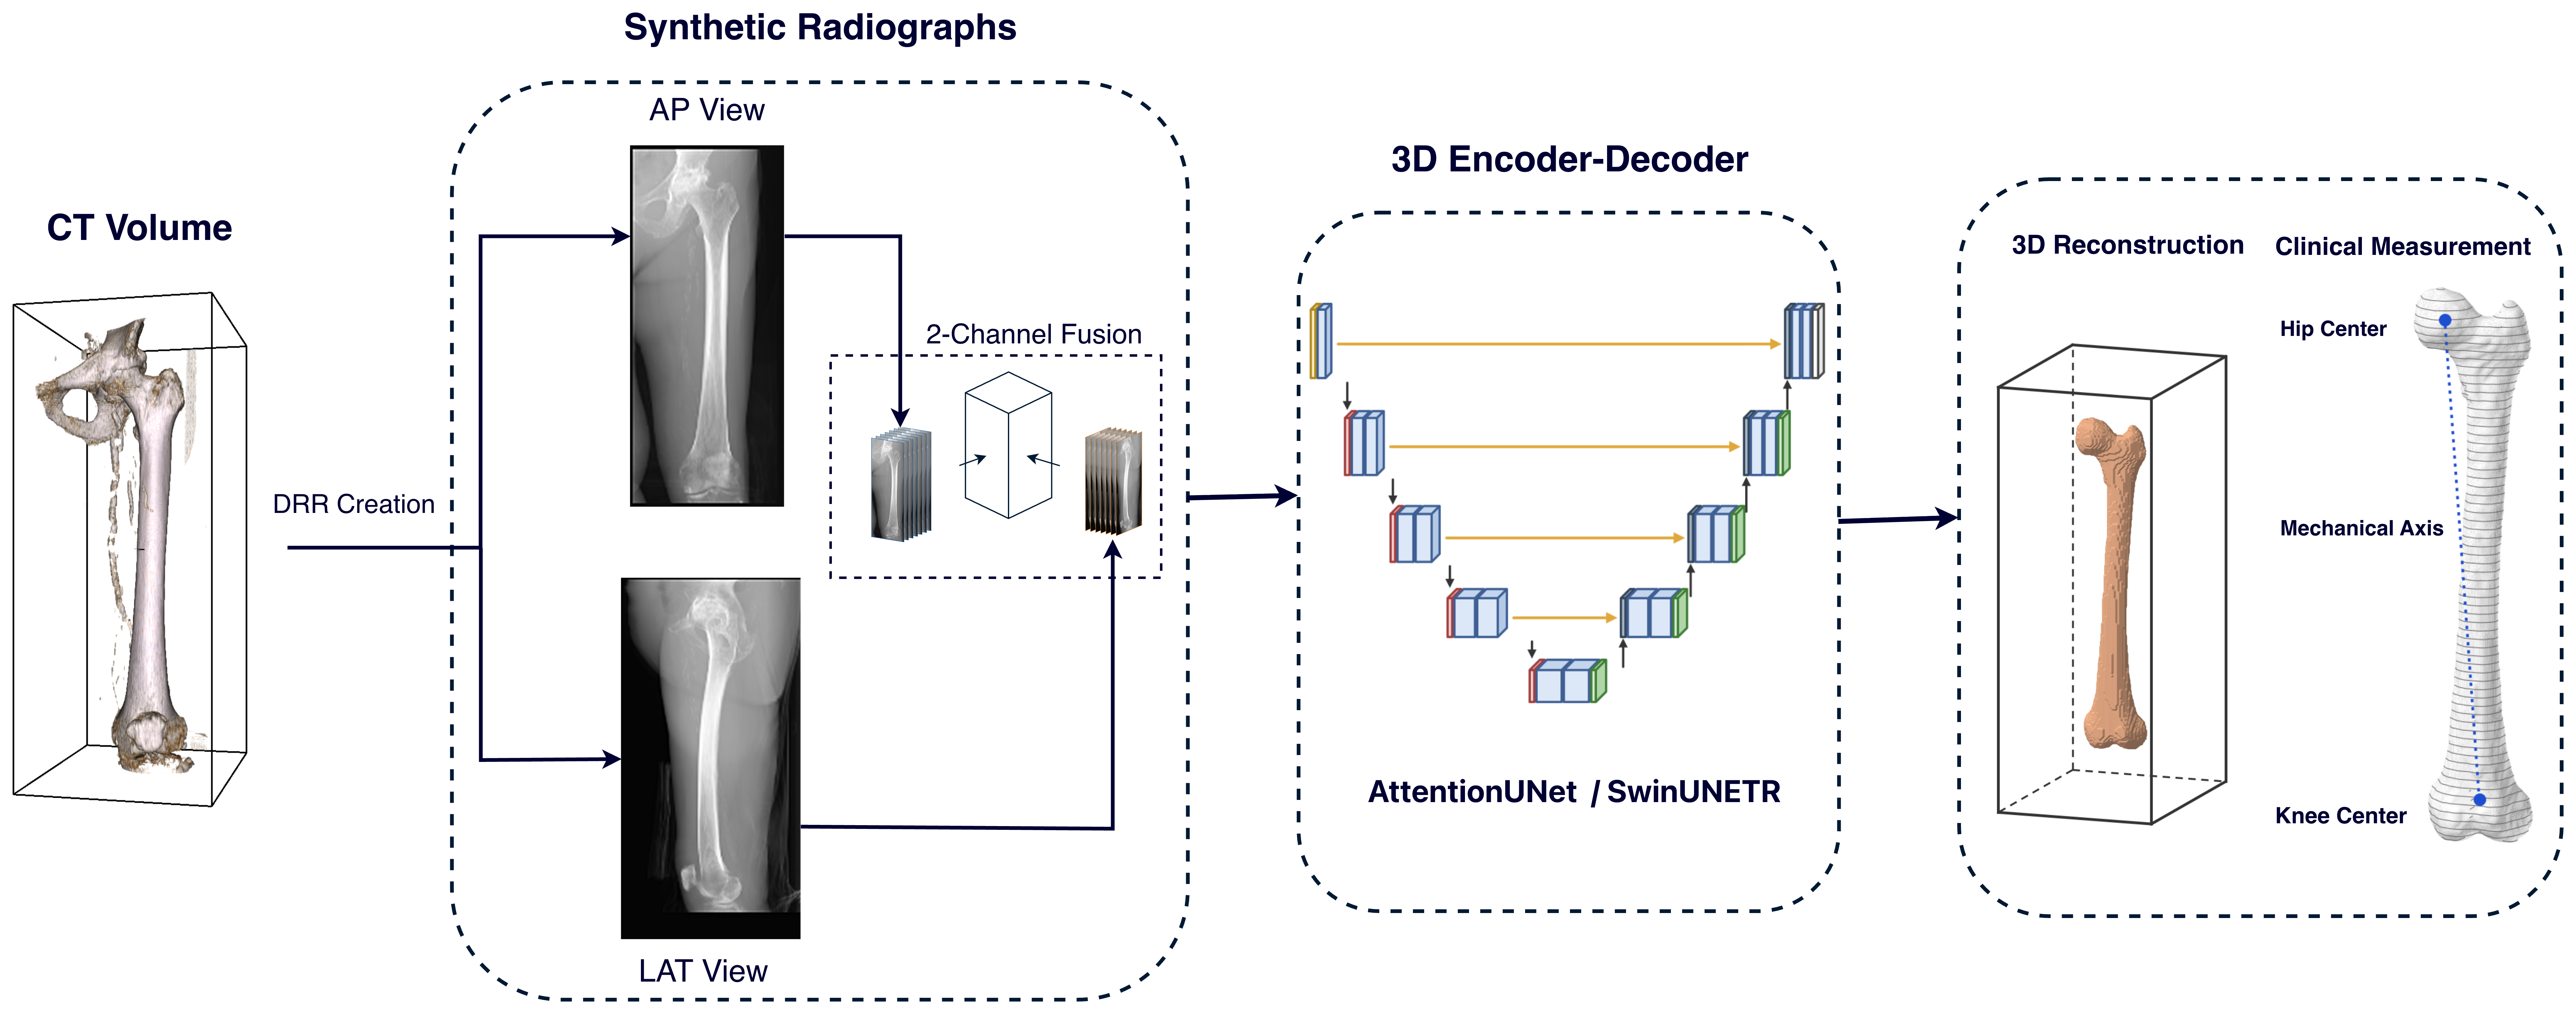
\includegraphics[width=\linewidth]{figures/pipeline.png}

  \vspace{0.5em}
  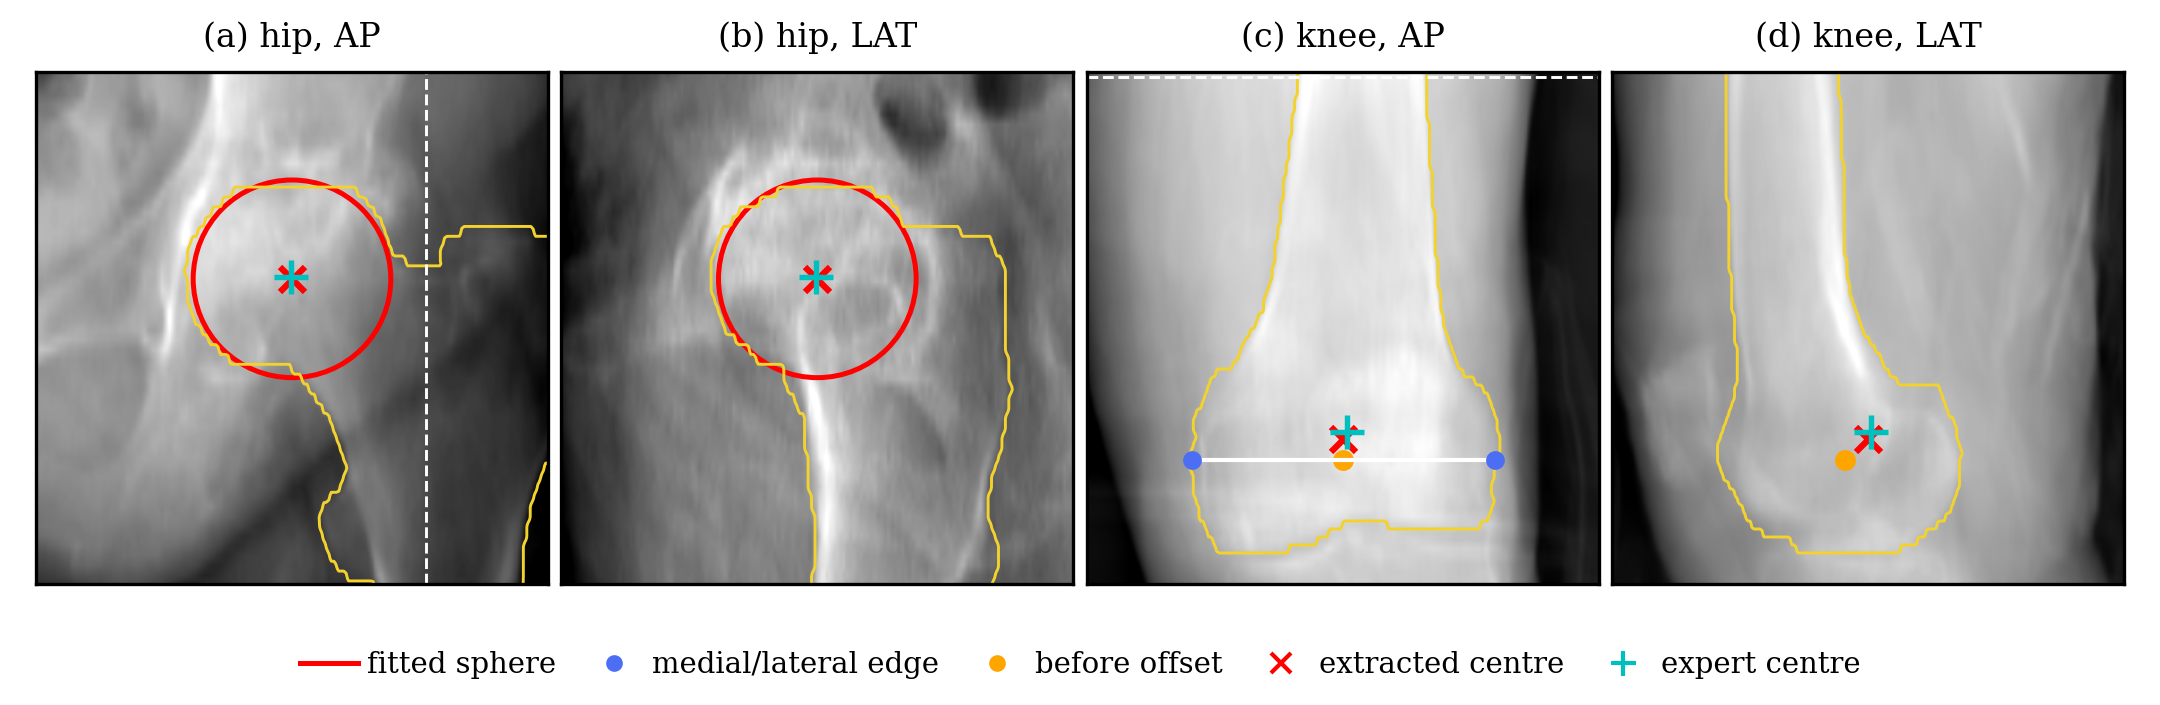
\includegraphics[width=\linewidth]{figures/landmarks.png}
}

% ---------------------------------------------------------------- column 2
\column{0.36}
\block{1. Median Dice hid the failures that mattered}{
  \claim{Nearly the same median Dice (0.930 vs 0.934), but 9 vs 0 femoral-head failures ($>$20\,mm).}
  \centering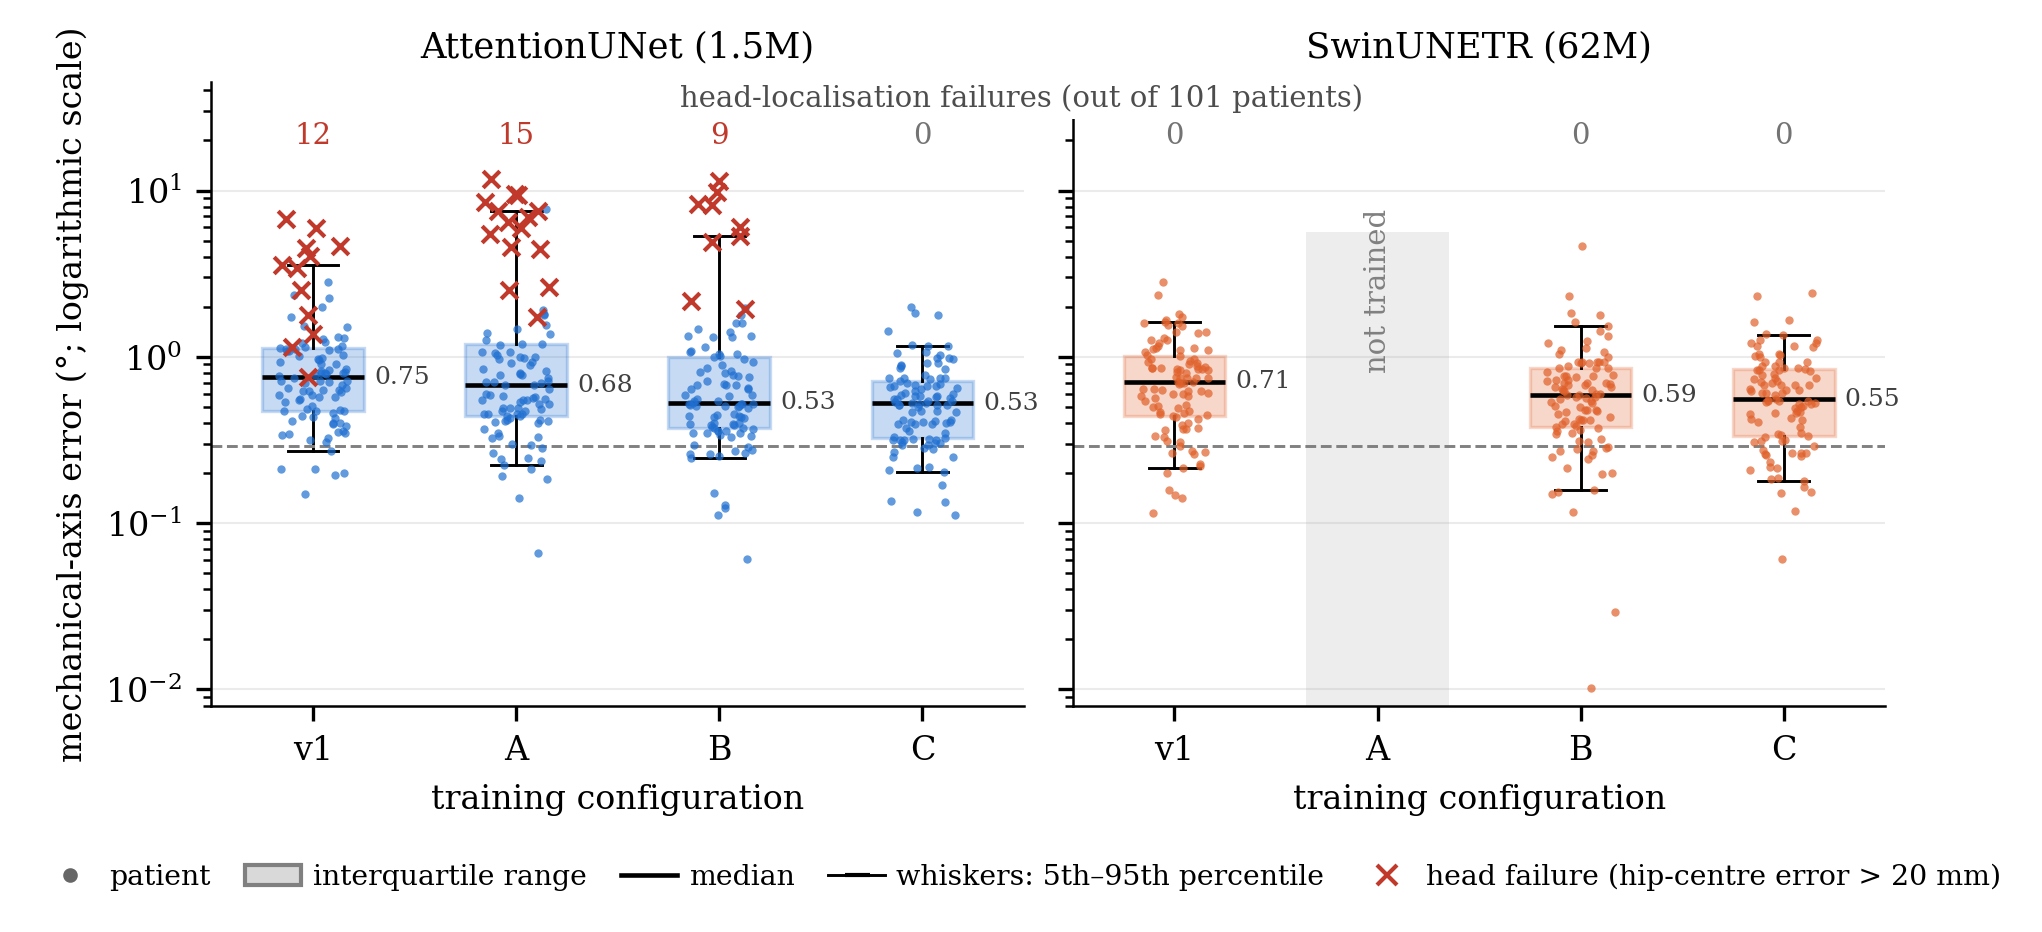
\includegraphics[width=0.86\linewidth]{figures/config_boxplot.png}

  \vspace{0.5em}
  \raggedright
  Configuration C (pose augmentation with re-projected radiographs, wider intensity augmentation, per-image
  normalisation) removed all nine failures. Then the
  \textbf{1.5M CNN matched the 62M transformer}: axis 0.53$^\circ$ vs 0.55$^\circ$, paired difference
  $-0.01^\circ$ [95\% CI $-0.13$, 0.03].

  \vspace{0.5em}
  \centering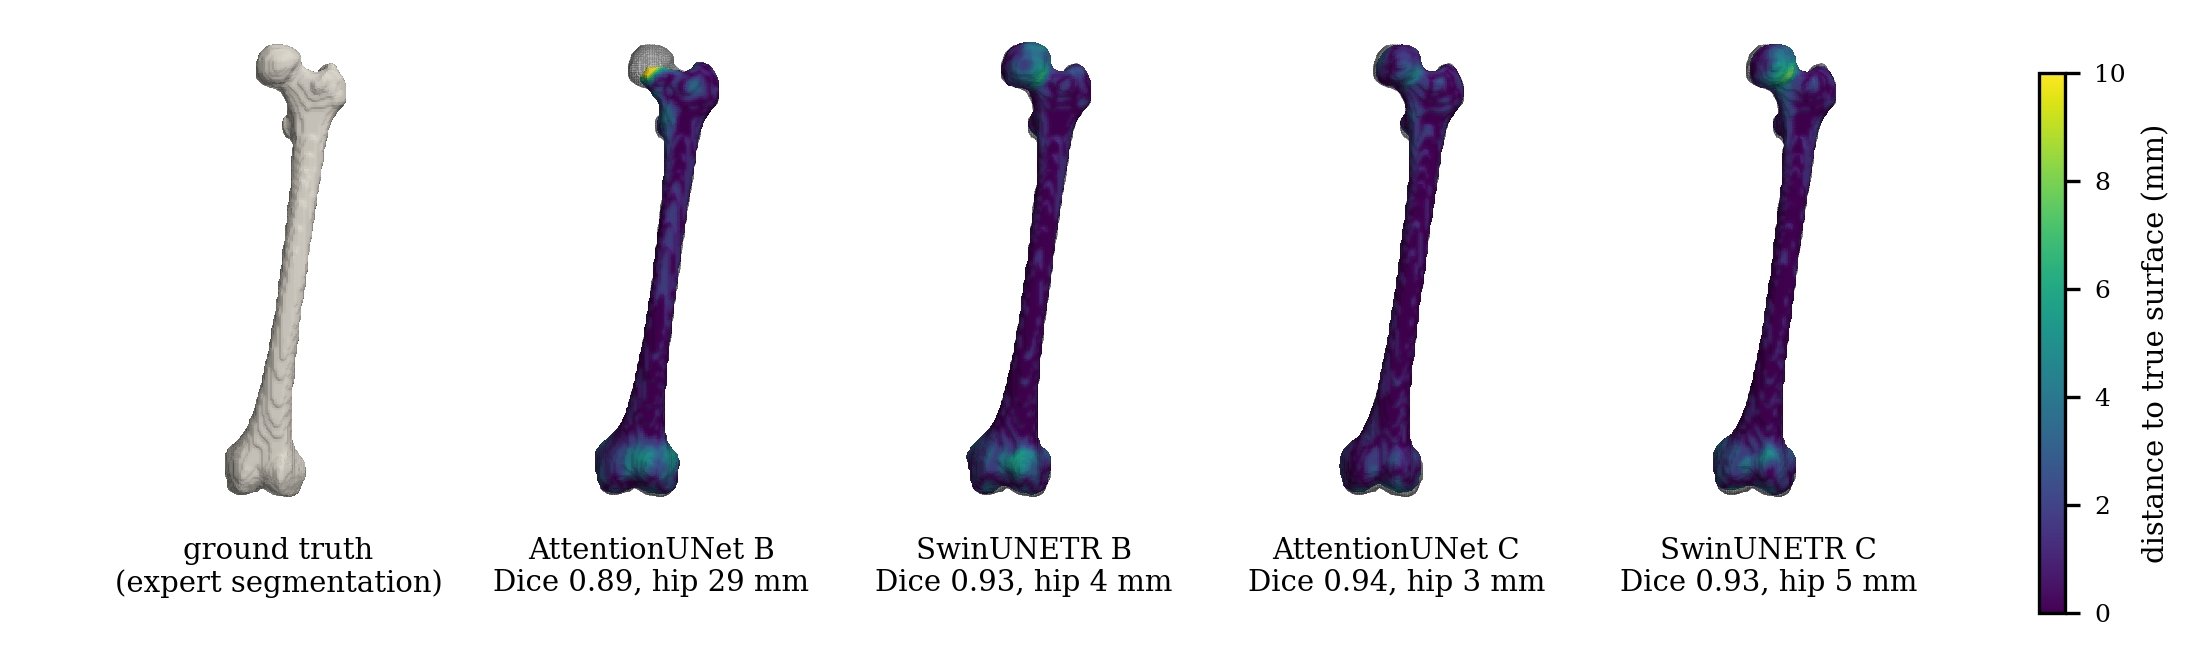
\includegraphics[width=0.86\linewidth]{figures/reconstruction_3d.png}\\
  {\normalsize Same case: AttentionUNet B misses the head (Dice 0.89, hip 29\,mm); configuration C fixes it.}
}

\block{Accuracy against experts}{
  \centering\large
  \renewcommand{\arraystretch}{1.1}\setlength{\tabcolsep}{14pt}
  \begin{tabular}{@{}lcc@{}}
    \toprule
    & HFValid (CV) & VSD (external) \\
    \midrule
    Axis error, AttentionUNet & 0.53$^\circ$ & 0.69$^\circ$ \\
    Axis error, SwinUNETR     & 0.55$^\circ$ & 0.62$^\circ$ \\
    Floor (true masks)        & 0.29$^\circ$ & 0.38$^\circ$ \\
    Head failures             & 0/101, 0/101 & 8/58, 6/58 \\
    \midrule
    Two experts disagree (VSD) & 0.30$^\circ$ & -- \\
    One expert vs consensus   & -- & 0.21$^\circ$ \\
    \bottomrule
  \end{tabular}

  \vspace{0.5em}
  About \textbf{1.8$\times$ expert disagreement} in CV, about 3$\times$ externally; 7/19 and 6/19 external femurs
  exceed 2$^\circ$.
}

% ---------------------------------------------------------------- column 3
\column{0.34}
\block{2. Extra error comes mainly from the hip}{
  \claim{Image-based methods misplace the femoral head 4.3--5.5$\times$ more than experts disagree.}
  \centering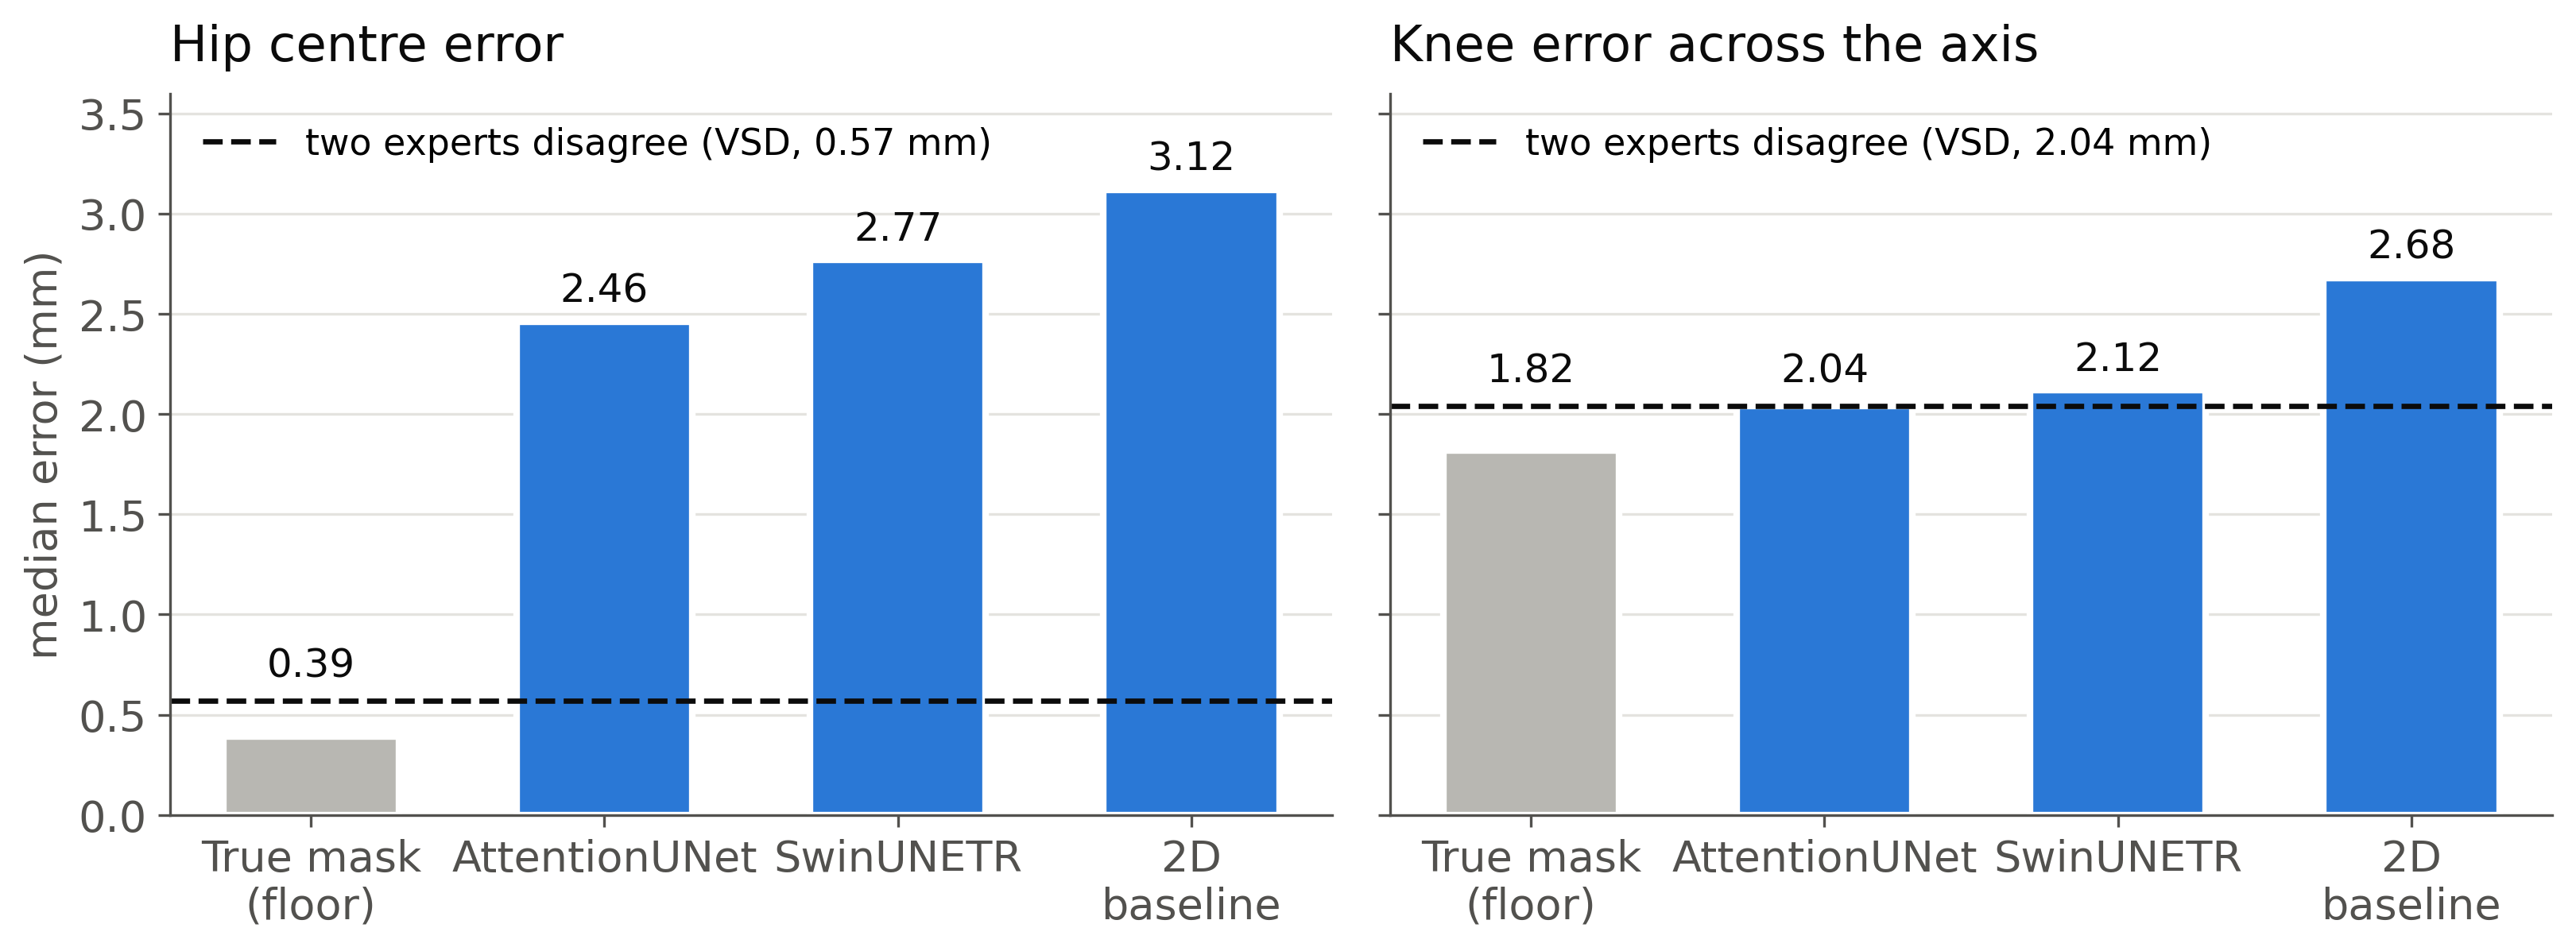
\includegraphics[width=\linewidth]{figures/poster_error.png}

  \vspace{0.5em}
  \raggedright
  \begin{itemize}
    \item The knee error lies mostly \textbf{along} the femur, which barely tilts the axis. A learned knee extractor
      cut it by 0.8--1.0\,mm; the axis did not change ($p\ge0.35$).
    \item The hip error is a \textbf{scatter, not a bias}, and the reconstructed head has no detectable size
      difference: right size, wrong place.
  \end{itemize}
}

\block{3. 2D detection vs 3D reconstruction}{
  A 2D network that finds the landmarks directly on both views reached \textbf{0.62$^\circ$} on HFValid
  (AttentionUNet 0.53$^\circ$, $p_\mathrm{Holm}=0.002$) and 0.61$^\circ$ externally (no significant difference).

  \vspace{0.5em}
  \claim{Choosing the epoch on the test fold made the same 2D network look 0.16$^\circ$ better (0.46$^\circ$).}
  Model selection alone moved the result by a quarter of the error. The 3D models (0.53$^\circ$, 0.55$^\circ$) were
  also selected on the test fold (by Dice), so this comparison favours them.
}

\block{Take-aways}{
  \begin{enumerate}
    \item To improve the axis, \textbf{place the femoral head more precisely}; a better knee rule did not help,
      and neither did a 41$\times$ larger network.
    \item Report failure counts and clinical errors, not only median Dice.
    \item Match training configurations before comparing architectures.
    \item Model inference runs without a GPU: Raspberry Pi~4, about 110\,s per case.
  \end{enumerate}
  \vspace{0.3em}
  {\normalsize Limitations: synthetic parallel-beam radiographs, one training cohort, 19 external femurs with landmarks,
  3D checkpoints selected on the held-out fold.}
}

\end{columns}
\end{document}
